%!TEX root = ../../report.tex
\section{Summary}
In this chapter various different methods of including pose estimation noise into the mapping has been evaluated. The method that was ultimately chosen was in ideal sensor model but with reduced certainty for each observation. The occupancy values chosen for free is \(0.4\) and \(0.6\) for occupied. The pose estimation noise in incorporated as a weight that reduces the certainty as the estimation variance increases. The weight calculation can be seen in equation \ref{eq:pose-weight}. 
These elements has been inserted in the static mapper block, as seen in figure \ref{fig:static_map_detail}. 
The sensor input and pose estimation is combined and inserted in the static map as determined by the sensor model and noise weight. At fixed intervals the static map is then provided as a snapshot as output and cleared. 

\begin{figure}[htbp]
	\centering
	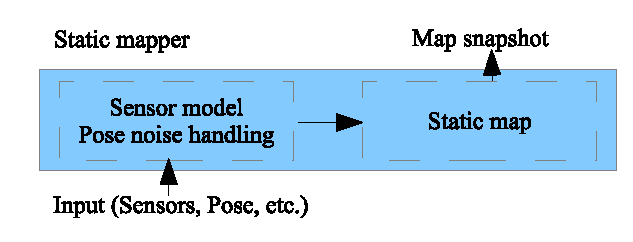
\includegraphics[scale=1]{chapters/static_mapping/figures/static_map_detail.eps}
	\caption{Static mapping module concept}
	\label{fig:static_map_detail}
\end{figure}

